\documentclass{beamer}
\usetheme{Warsaw}
\setbeamertemplate{footline}[frame number]

\usepackage[utf8]{inputenc}
\usepackage{fancybox}
\usepackage{multimedia} 
\usepackage{subfig}
\usepackage{amsmath}
\usepackage{hyperref}
\usepackage[all]{xy}
\begin{document}


\title[Angewandte Mathematik] % (optional, only for long titles)
{Angewandte Mathematik
\\
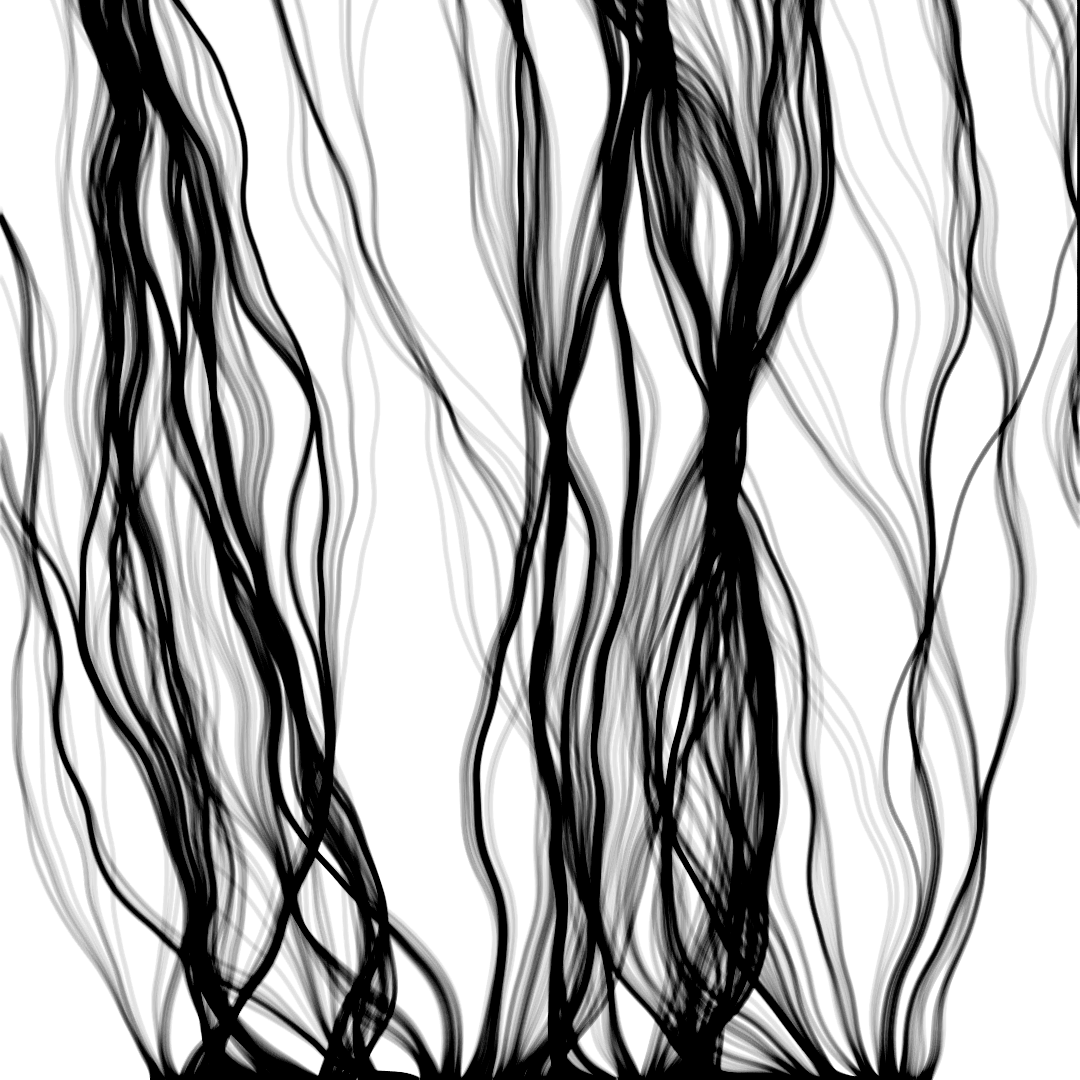
\includegraphics[scale=0.15]{images/cover}
}
\subtitle{}
\author[Dr. Johannes Riesterer] % (optional, for multiple authors)
{Dr.  rer. nat. Johannes Riesterer}

\date[KPT 2004] % (optional)
{}

\subject{Angewandte Mathematik}

\frame{\titlepage}

\begin{frame}
    \frametitle{Angewandte Mathematik}
\framesubtitle{}
    \begin{block}{Kann jeder Mathematik lernen?}
\begin{itemize}
 \item Mathematik hat ein Motivationsproblem
\item Jeder kann Mathematik lernen, aber Mathematik unterrichten ist sehr schwer, da jeder individuelle Materialien braucht.
 \item Eigeninitiative ist nötig/KI Verwenden

\end{itemize}
\end{block}

 \end{frame}


\begin{frame}
    \frametitle{Angewandte Mathematik}
\framesubtitle{}
    \begin{block}{Konstruktivismus}
Die Existenz mathematischer Objekte ist durch ihre Konstruktion zu begründen. 
\end{block}
    \begin{block}{Platonismus}
Mathematische Gegenstände (Zahlen, geometrische Figuren, Strukturen) und Gesetze sind keine Konzepte, die im Kopf des Mathematikers entstehen, 
sondern es wird ihnen eine vom menschlichen Denken unabhängige Existenz zugesprochen.
\end{block}

\begin{figure}[H]
    \centering
  
\includegraphics[width=0.25\textwidth]{images/hardchoice.png}
    \caption{}
\end{figure}
 \end{frame}


\begin{frame}
    \frametitle{Angewandte Mathematik}
\framesubtitle{}
    \begin{block}{Was ist (angewandte) Mathematik?}
\begin{itemize}
\item Algorithmen zum Lösen von Problemen.
 \item Abschätzungen, wie gut und genau die Algorithmen funktionieren.
 \item Mathematische Grundlagen, auf denen Algorithmen und Abschätzungen basieren. 
 \item Softwaretechnische Aspekte in Bezug auf  Implementierung der Algorithmen.
\end{itemize}
\end{block}
 \end{frame}

\begin{frame}
    \frametitle{Angewandte Mathematik}
\framesubtitle{}
    \begin{block}{Mathematische Modellierung}
\begin{figure}[H]
      \centering
    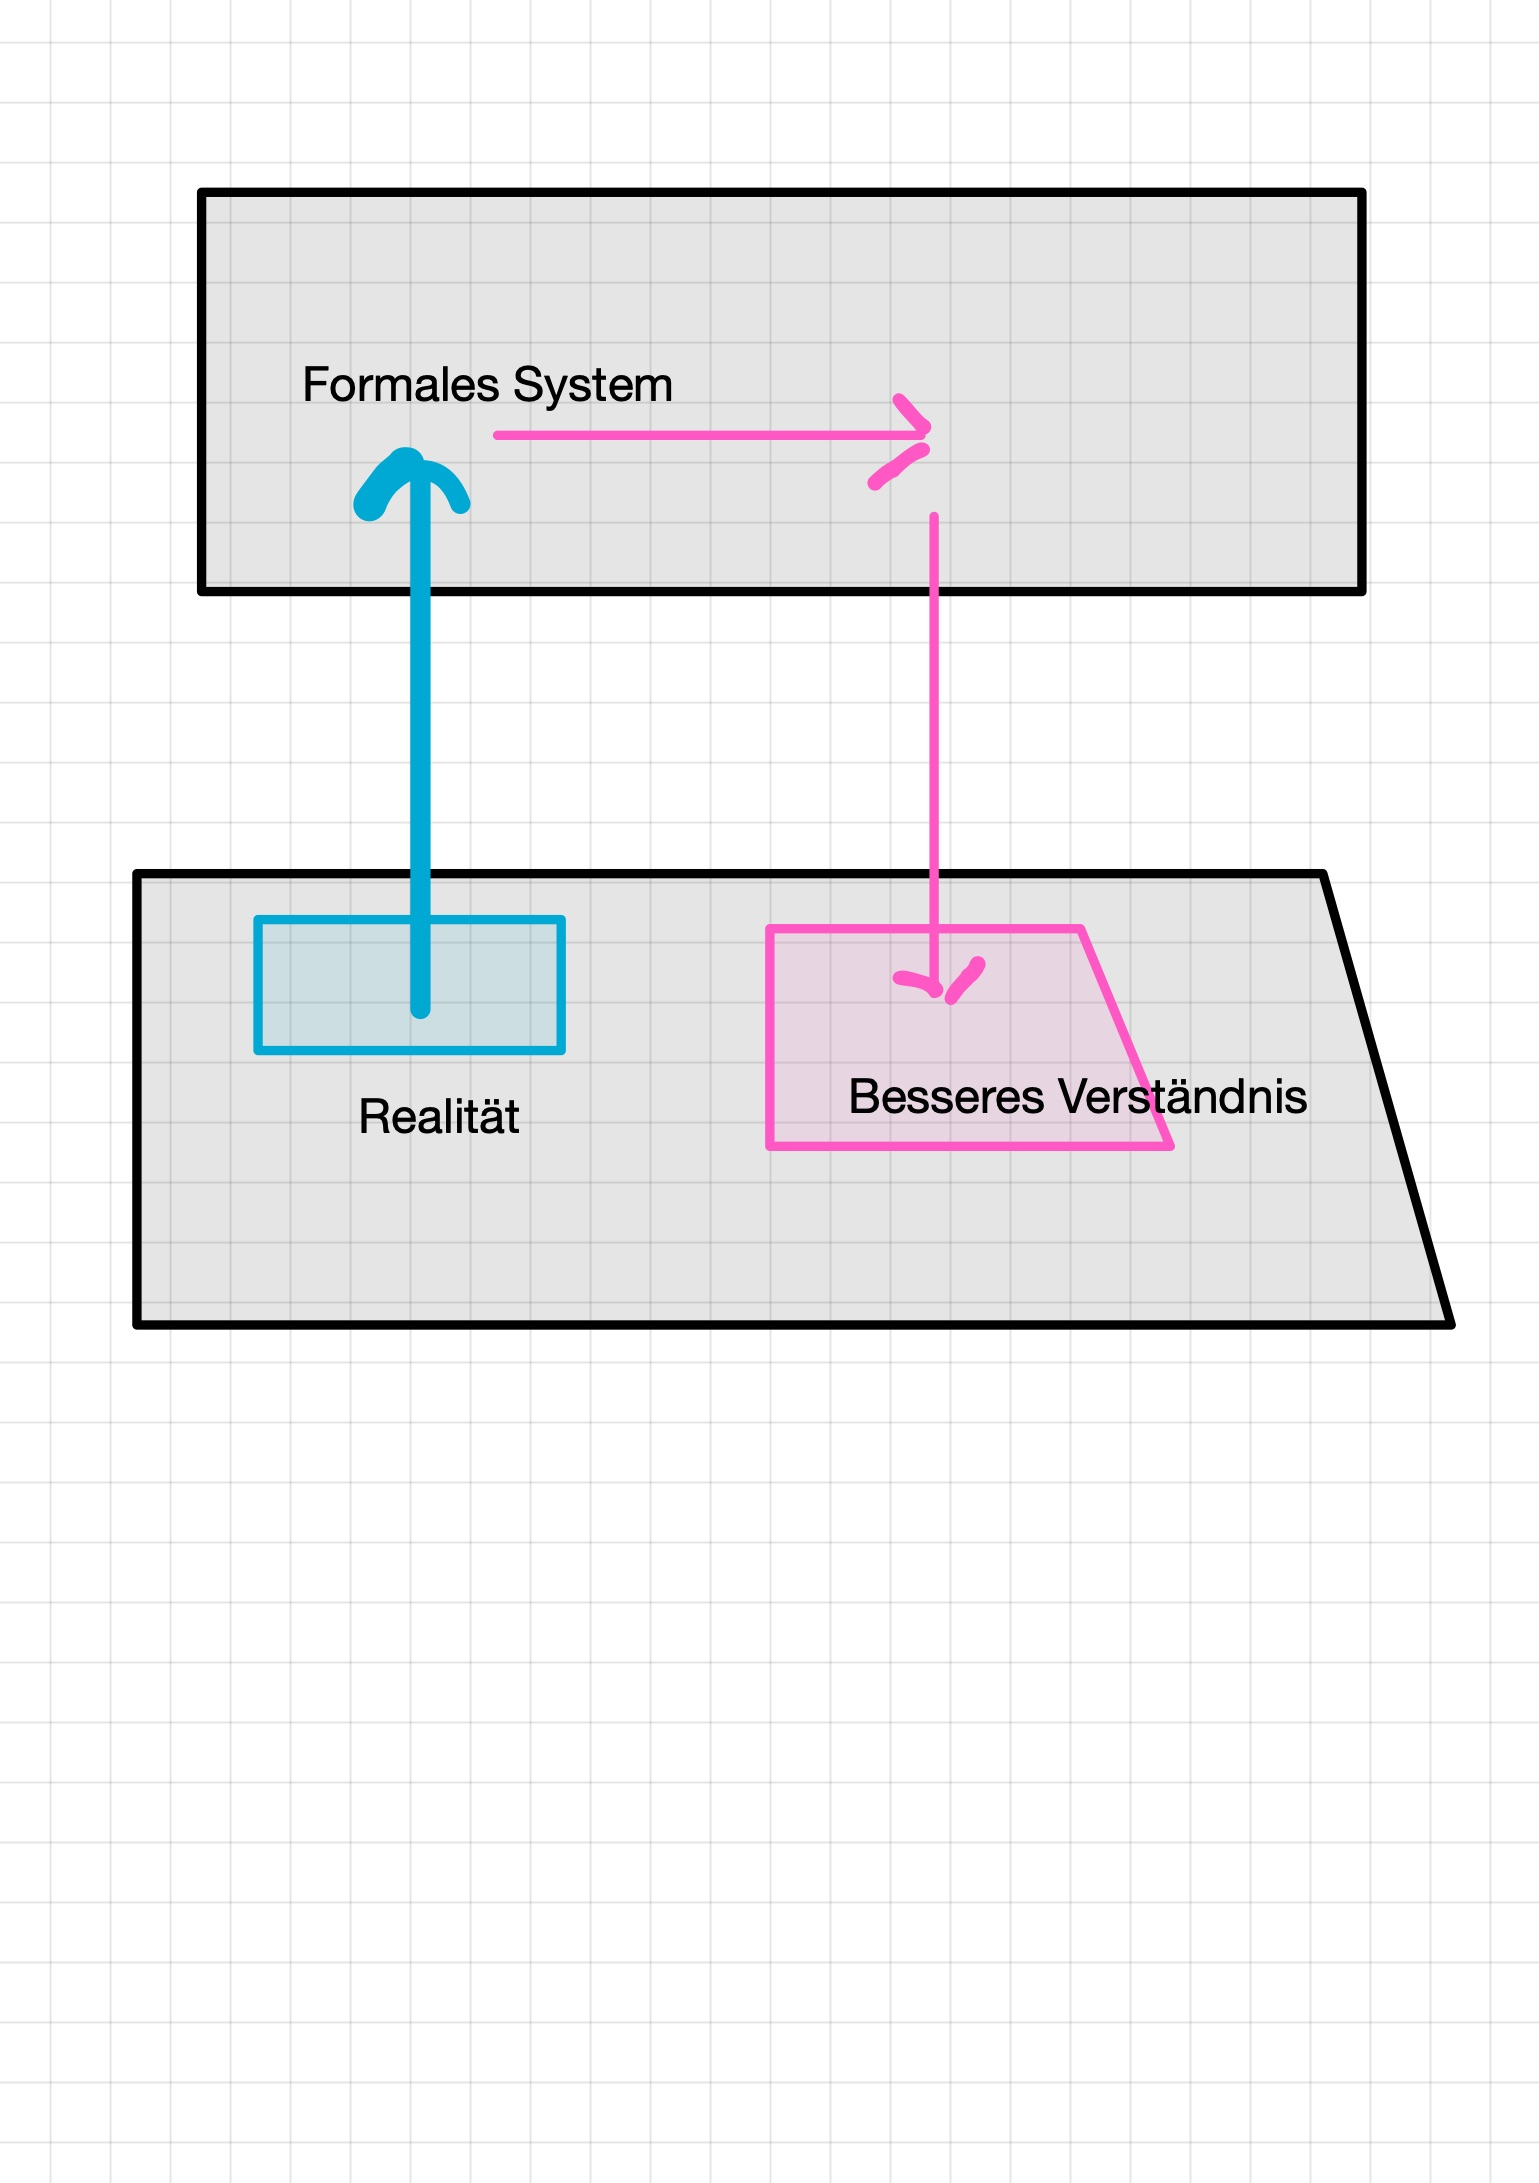
\includegraphics[width=0.7\textwidth]{images/modellierung}
      \caption{Quelle: Wikipedia: }
\end{figure}
\end{block}
 \end{frame}


 \begin{frame}
    \frametitle{Angewandte Mathematik}
\framesubtitle{}
    \begin{block}{Formale Systeme}
\begin{itemize}
\item Mengenlehre (Logik erster Stufe)
\item Kategorientheorie
\item Typentheorie
\end{itemize}
\end{block}
 \end{frame}



 \begin{frame}
    \frametitle{Angewandte Mathematik}
\framesubtitle{Themen}
    \begin{block}{Themen}
        Wir werden in der Vorlesung die folgenden Themen behandeln:
        \begin{itemize}
            \item Computergestützte Beweissysteme
            \item Numerische Software
            \item Mehrdimensionale Differentialrechnung
            \item Differentialgleichungen und ihre numerische Lösungen
            \item Qualtität von numerischen Lösungen
            \item Optimierungsverfahren und neuronale Netze
        \end{itemize}
    \end{block}
 \end{frame}


\end{document}

